\section{What are the different techniques, mechanisms and tools the MediaGenix company
uses to automate repetitive development work?}

\begin{itemize}
\item Model-Driven Development approach. This approach allows to automate generation of code (DB creation scripts, UI forms, ...) by describing an abstraction of a model (called SuperModel).
    \begin{itemize}
    \item Automation of DB installation.
    \item Automation of UI building.
    \end{itemize}
\item Automated testing
    \begin{itemize}
    \item JUnit and SUnit to writte unit tests for Java and SmallTalk.
    \item Acceptance tests: End-to-end tests, testing the software from the end-user point of view.
    \item Integrated into IDE.
    \item Writte tests once, reuse many times.
    \end{itemize}
\end{itemize}


\section{The entire development of MediaGenix WHATS'On software product (line) is done in
the Smalltalk language.
Why did the company decide to use Smalltalk?
What are the acclaimed advantages of Smalltalk to develop software products?
What features of Smalltalk make it a good language to automate repetitive work?}

The company decides to use Smalltalk because it has very interesting features : 

\begin{itemize}
\item Easy to read
\item Smalltalk is written in itself
\begin{itemize}
\item Classes
\item Methods
\item Compiled code
\end{itemize}
\item All these objects can be accessed by your own code
\item Very good reflection capabilities
\item Incremental compilation (Smalltalk system is "alive", your code is \textbf{always} running so code changes take effect immediately
\item No compilation/build wait times
\item Easy to dynamically generate code
\item Used for performance tuning
\item Has its garbage collector
\item Has a good debugger
\end{itemize}


\section{To build their WHATS’On product (line) MediaGeniX strongly relies upon a modeldriven
development approach.
Explain with an example and in your own words.
Why do they follow such a model-driven development approach?}

In the Model-Driven development approach, we use meta information about domain model to automate tasks and to promote reuse.

The principle is that we write an abstraction of a model. 
This abstraction is written using a model language (like a Domain Specific Language).
Then, the abstraction is used to generate artifacts that are used by the application: GUI, model, DB mapping, ...

\subsection{Example (from the slides)}
We want to create a \textit{Person} with
\begin{itemize}
\item User interface for editing
\item Storage in relational DB
\item Possibility to export as XML file
\end{itemize}

\begin{table}[!ht]
\centering
\begin{tabular}{|ll|}
\hline
\multicolumn{2}{|l|}{Person} \\ \hline
firstName     & String     \\
lastName      & String     \\
birthDate     & Date       \\
isMarried     & Boolean    \\ \hline
\end{tabular}
\caption{\textit{Person} model}
\label{MDD:personmodel}
\end{table}

Here is how the Super model is written in SmallTalk:

\begin{lstlisting}
Person>>buildSuperModelWith: aBuilder

aBuilder
  dbTableName: 'Person';
  xmlTagName: 'Person'.
  
aBuilder
  addString: #firstName dbName: 'firstName' uiName: 'Voornaam' xmlTag: 'firstName';
    beMandatory;
  addString: #lastName dbName: 'lastName' uiName: 'Familienaam' xmlTag: 'lastName';
    beMandatory;
  addDate: #birthDate dbName: 'birthDate' uiName: 'Geboortedatum' xmlTag: 'birthDate';
  addBoolean: #isMarried dbName: 'isMarried' uiName: 'Getrouwd' xmlTag: 'isMarried' initialValue: false
\end{lstlisting}

From the code above, the database creation scripts are generated as well as the mapping operations (Create, Read, Update, Delete).
The User Interface to edit a \textit{Person} is also generated as well as the XML generation process.

\subsection{Why do they follow such a model-driven development approach?}
Thanks to Model-Driven development approach, we observe the following advantages:
\begin{itemize}
\item Faster development: the model is more abstract and is automatically transformed to a working application.
\item Leads to increased quality: the quality of the code depends on the engine used to generate it. It is easier to be extra carreful when writting a generator once than being always carreful when writting code.
\item Customization is easy: if a client wants to add a field somewhere, you just extends the model, add the field and the generated application will reflect the changes.
\end{itemize}


\section{Would you consider the WHATS'On software system created by MediaGenix as a
standard application, a library or rather an application framework? Explain.}

Application framework
%As reminder, an application framework is :
%\begin{itemize}
%\item an object oriented class hierarchy
%\item plus a build-in model of interactions 
%\item which defines how objects derived from the class hierarchy interact with one another
%\end{itemize}
%Deriving a custom application from a framework is typically done through class specialisation

The core functionality of WHAT's On is implemented as set of abstract classes that cooperate in a well-defined manner. (The software base product)
When deriving a concrete application (for a particular customer): these abstract classes are specialised by concrete subclasses and
other concrete classes are chosen from a library of standard 
components provided by the framework developer (SuperModel). 
Customisation is completed by adding new application-specific classes.


%\todo[inline]{Réponse par Zélie Mulders}

\section{Do there exist different variations of the WHATS’On application created by MediaGenix,
for its different clients?
What implementation techniques are used for implementing the different variations of
the product among its different clients?}
Yes, WHATS'On is a software product that can be extended with a new customisation for each client (they have approximately 30 customers wanting new stuff).
%They used a group of software development methodologies. Principally, they use agile development: ask customer what he wants, regularly show him  what you made, conitnuously  ask his feedback. So in the end, the customer gets what he wants.
%??? Implementations techniques VS Development techniques ??

They use \textit{Model-Driven Development} approach.
With this approach, they use inheritance to add customer specific behavior (for example if the customer wants a new field for the Person model, they just extend the previous PersonModel to a new PersonNewCustomerModel). 
\begin{center}
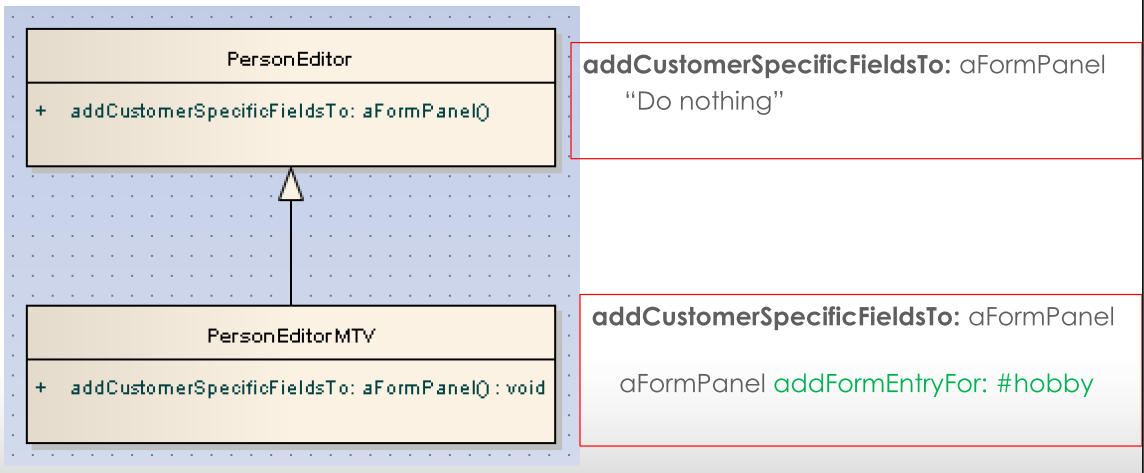
\includegraphics[width=0.5\textwidth]{customerLayout.PNG}
\end{center}


\section{How important is testing to the MediaGenix company, and why?
What testing techniques and which different kinds of tests do they use?
How does MediaGeniX automate its testing process?
What is the (positive and negative) impact of tests on maintenance?}

It is very important for them and used to garantee that their software keeps on running when changes are made to the code. 
WIth manual testing, they should do repetitive work (1,6 millions lines of code testing and more than 30 customers to tests). So they use automated testing. They have more than 1300 TestCase classes (in JUnit or SUnit).
They do 
\begin{itemize}
\item \textbf{Acceptance tests : } Test the application logic from the point of view of an end user. No individual methods. Complete flow from user interface to database and back.
\item \textbf{Typical scenario testing : } Set up initial data. Assert that the condition you are going to test is \emph{NOT} met. Do some stuff. Assert that the condition you are going to test \emph{IS} met.
\item \textbf{Regression tests : } If someone inadvertently changes behavior, the tests should detect it.
\end{itemize}
Automated tests are crucial because you cannot manually test a large application. They have more than 20.000 automated tests (which takes 8hours to run). But they used parallel execution on 16 computers to get the results in 30 minutes.
Automated testing demands extra works and represents 30\% of the total source code. So they have an impact on the development time (almost double the development time). Moreover, the tests need to be maintained. If a functionality changes, tests need to be changed.
However, testing pay back in the long run. You write them once and you can reuse them many times.

%\todo[inline]{Réponse par Zélie Mulders}
